\section{Refinement-based game semantics}

This section introduces the category $\mathcal{G}$ of games and strategies
we use to interpret the behavior of low-level interacting components.
$\mathcal{G}$ has no high-order structure,
which simplifies the definition of games considerably.
On the other hand,
our definition of strategy is generalized to accomodate specifications,
and the morphisms of $\mathcal{G}$ are equipped with a notion of refinement
suitable for our purposes.

\subsection{Behavior specifications}

Before we introduce games and strategies
in the following sections,
we define the \emph{behavior specification} monad $\mathcal{B}$
which captures our treatment of
silent divergence, undefined behaviors, and non-determinism,
as well as the associated notion of refinement.

\subsubsection{Divergence} %{{{

[XXX update]

We model internal actions in the following way.
Whenever $\kw{P}$ is to play,
it may instead perform an internal action ($\tau$),
in which case $\kw{P}$ will retain control.
There is no limit on the number of internal actions that
$\kw{P}$ may perform before playing a move;
we say that a strategy \emph{diverges}
when it performs internal actions indefinitely.

Internal actions usually correspond to the hidden interactions
within composite systems, and
divergence is an \emph{emergent} phenomenon:
systems that are well-behaved when taken in isolation
may nontheless exhibit divergence when they interact with one another.
As such,
divergence is one of the major sources of complexity
in compositional semantics.

In our setting,
the occurence of internal actions
is observable,
and our definition of simulation
makes no effort
to identify finite sequences of internal actions
which have different lengths.
Instead,
in \S\ref{sec:bigstep}
we introduce an operator $- \backslash \tau^*$
that can be used to normalize strategies
by eliminating altogether all such finite sequences.

%}}}

\subsubsection{Undefined behaviors} %{{{

Low-level language semantics and specifications
often contain \emph{undefined behaviors}:
there are circumstances under which the behavior of the system
is entierly unrestricted;
any execution that reaches such circumstances is said to ``go wrong''.
We model this using the special outcome $\lightning$
representing a computation whose behavior is undefined
from that point on.

The undefined behavior can be implemented by anything,
but can only implement itself;
as such,
$\lightning$
acts as a greatest element with respect to refinement.

%}}}

\subsubsection{Non-determinism} %{{{

[of the system's specification,
expresses the range of behaviors that are allowed]

%}}}

\subsubsection{Monad}

The notion of computation outlined above
yields the following definition
for the behavior specification monad:
\[
    \mathcal{B}(X) := \mathcal{P}(X + \{\Delta\})^\lightning
\]
That is,
computations are a sets of possible outcomes (values or silent divergence),
which we augment with a special computation $\lightning$
intended as a greatest element for refinement.

The unit of $\kw{ret}_A : A \rightarrow \mathcal{B}(A)$
of the monad $\mathcal{B}$ is given by:
\[
    \kw{ret}_A(a) = \{ a \} \,,
\]
and the binding operation is defined by the rules:
\[
    \AxiomC{$x \ni a$}
    \AxiomC{$f(a) \ni b$}
    \BinaryInfC{$(x \bind f) \ni b$}
    \DisplayProof
    \quad
    \AxiomC{$x \ni \Delta$}
    \UnaryInfC{$(x \bind f) \ni \Delta$}
    \DisplayProof
    \quad
    \AxiomC{}
    \UnaryInfC{$(\lightning \bind f) \ni \lightning$}
    \DisplayProof
\]
The usual monad laws hold:
\begin{align*}
    \kw{ret}(v) \bind f &= f(v) \\
    x \bind \kw{ret} &= x \\
    x \bind (v \mapsto f(x) \bind g) &= (x \bind f) \bind g
\end{align*}

Recall that the Kleisli category associated with the monad $\mathcal{B}$
has sets a objects and
functions of type $f : A \rightarrow \mathcal{B}(B)$
as its morphisms $A \leadsto B$ between sets $A$ and $B$.
For $f : A \leadsto B$ and $g : B \leadsto C$,
the Kleisli composition $f \cdot g : A \leadsto C$
and its identity $\mathbf{1}_A : A \leadsto A$ are defined as:
\[
    f \cdot g := a \mapsto f(a) \bind g \qquad \mathbf{1}_A := \kw{ret}_A \,.
\]
In the remainder of this section we show that
the Kleisli category associated with $\mathcal{B}$
can further be equipped with a structure analogous
to a typed Kleene algebra.

\subsubsection{Refinement}

We can promote a relation $R : \mathcal{R}(A, B)$
to behavior specifications in the following way:
\[ \mathcal{B}^+(R) :=
   \mathcal{P}^+(R + \{ (\Delta, \Delta) \})^\lightning \]
We will use:
\[ {\sqsubseteq}_A := \mathcal{B}^+(=_A) \]
as our notion of refinement.

The relation lifting operator $\mathcal{B}^+$ defines a \emph{relator},
so that the following properties hold:
\begin{gather*}
  {=}_{\mathcal{B}(X)} \subseteq \mathcal{B}^+(=_X) \\
  \mathcal{B}^+(R) \cdot \mathcal{B}^+(S) \subseteq
    \mathcal{B}^+(R \cdot S) \\
  R \subseteq S \Rightarrow
    \mathcal{B}^+(R) \subseteq \mathcal{B}^+(S) \,.
\end{gather*}
In particular, $\mathcal{B}^+(R)$ is compatible with $\sqsubseteq$
in the following sense:
\[
    {\sqsubseteq} \cdot \mathcal{B}^+(R) \:\subseteq\: \mathcal{B}^+(R) \qquad
    \mathcal{B}^+(R) \cdot {\sqsubseteq} \:\subseteq\: \mathcal{B}^+(R)
\]
Furthermore the monad operations satisfy the expected relational properties,
summarized in Fig.~\ref{fig:monadr}.
[known as "lax extension", monad relator]

The refinement partial order $\sqsubseteq_A$
defines a complete lattice on $\mathcal{B}(A)$.
Given $x, y : \mathcal{B}(A)$,
their supremum $x \vee y : \mathcal{B}(A)$
can be interpreted as a non-deterministic choice
between the computations $x$ and $y$,
or as the specification that permits the behavior of either.
On the other hand $x \wedge y : \mathcal{B}(A)$ can be interpreted as
the specification requiring that $x$ and $y$ both be satisfied.
The least element $\varnothing$
is a specification that can never be satisfied;
the greatest element $\lightning$
is the specification that is always satisfied.

This lattice structure
can be extended pointwise to Kleisli morphisms.
In particular, for $f : A \leadsto B$ and $g : A \leadsto B$,
we define $f + g : A \leadsto B$ and $\mathbf{0}_{A,B} : A \leadsto B$ as:
\[
  f + g := a \mapsto f(a) \vee g(a) \qquad
  \mathbf{0}_{A,B} := a \mapsto \varnothing \,.
\]

\begin{figure}
  \begin{gather*}
    R : \mathcal{R}(A_1, A_2),
    S : \mathcal{R}(B_1, B_2),
    T : \mathcal{R}(C_1, C_2) \\
    \kw{ret}_{A_1}
        \ifr{R \rightarrow \mathcal{B}^+(R)}
        \kw{ret}_{A_2} \\
    ({\bind})
        \ifr{\mathcal{B}^+(R) \rightarrow (R \rightarrow \mathcal{B}^+(S))
          \rightarrow \mathcal{B}^+(S)}
        ({\bind}) \\
    {\cdot}
        \ifr{(R \rightarrow \mathcal{B}^+(S)) \rightarrow
             (S \rightarrow \mathcal{B}^+(T)) \rightarrow
             (R \rightarrow \mathcal{B}^+(T))}
        {\cdot} \\
    \mathcal{B}(-)
        \ifr{(R \rightarrow S) \rightarrow
             \mathcal{B}^+(R) \rightarrow \mathcal{B}^+(S)}
        \mathcal{B}(-)
  \end{gather*}
  \caption{Relational properties for behavior specifications}
  \label{fig:monadr}
\end{figure}

\subsubsection{Iteration}

A Kleisli morphism of type $f : A \leadsto A$
can be interpreted as a transition relation on $A$,
and we define its non-deterministic iteration $f^*$
in the usual way:
\[
    f^* := \sum_{n \in \mathbb{N}} f^n \,,
\]
where $f^n$ is
the $n$-fold composition of the form $f \cdot f \cdots f$.
To account for divergence,
we also introduce the infinite iteration operation:
\[
    f^\omega := a \mapsto \{ \Delta \mid
      \forall n \in \mathbb{N} \,.\,
      f^n(a) \ne \varnothing \} \,,
\]
and define $f^\infty := f^* + f^\omega$.

The structure
$\langle A \leadsto B, {\cdot}, \mathbf{1}, {+}, \mathbf{0}, * \rangle$
is analogous to a typed Kleene algebra,
however it does not validate right-annihilation of $\cdot$ by $\mathbf{0}$.
In particular, note that:
\begin{gather*}
  \mathbf{1}^\infty \cdot \mathbf{0} =
    (a \mapsto \{ \Delta \}) \ne \mathbf{0} \\
  (a \mapsto \lightning) \cdot \mathbf{0} =
    (a \mapsto \lightning) \ne \mathbf{0} \,.
\end{gather*}

%\subsection{Left Kleene Categories}
%
%The properties of the behavior specification monad
%are captured by the following definition.
%
%\begin{definition}
%A \emph{left Kleene category}
%is a category $\mathbf{C}$ whose homsets $\mathbf{C}(A, B)$
%are equipped with the operations:
%\begin{gather*}
%  {+}_{A,B} :
%    \mathbf{C}(A, B) \times \mathbf{C}(A, B) \rightarrow \mathbf{C}(A, B) \\
%  0_{A,B} :
%    \mathbf{C}(A, B) \\
%  -^* :
%    \mathbf{C}(A, A) \rightarrow \mathbf{C}(A, A)
%\end{gather*}
%In addition to the usual properties of categories, whereby for
%$f : A \rightarrow B$, $g : B \rightarrow C$, and $h : C \rightarrow D$
%we have:
%\[
%   f \circ \kw{id}_A = \kw{id}_B \circ f = f \qquad
%   h \circ (g \circ f) = (h \circ g) \circ f \,,
%\]
%the additive structure is an idempotent commutative monoid:
%\begin{align*}
%   f_1 + f_2 &= f_2 + f_1 \\
%   (f_1 + f_2) + f_3 &= f_1 + (f_2 + f_3) \\
%   f + f &= f \,,
%\end{align*}
%and composition distributes over addition as follows:
%\begin{align*}
%  g \circ (f_1 + f_2) &= g \circ f_1 + g \circ f_2 \\
%  (g_1 + g_2) \circ f &= g_1 \circ f + g_2 \circ f \\
%  0 \circ f &= 0 \,.
%\end{align*}
%Finally, the iteration operation is characterized
%by the following conditions:
%\begin{align*}
%  1 + f \circ f^* \sqsubseteq f^* \\
%  1 + f^* \circ f \sqsubseteq f^* \\
%  g \circ f \sqsubseteq g \rightarrow g \circ f^* \subseteq g \\
%  f \circ g \sqsubseteq g \Rightarrow f^* \circ g \subseteq g
%\end{align*}
%A category is a left-Kleene category \emph{with infinite iteration} if,
%in addition,
%it has an operator $-^\omega$
%with the properties:
%
%
%
%\end{definition}
%
%
%with composition $\cdot$ and identities $\mathbf{1}$
%
%
%
%However, as noted in \cite{failkat},
%the possibility of an abnormal outcome
%means that annihilation of $\cdot$ by $0$ on the right
%does not hold in general.
%In particular, defining :
%Likewise,
%
%
%Nevertheless,
%this notion of iteration
%and the associated equational theory
%will be useful
%for defining strategies operationally,
%in terms of small-step transition relations.
%
%%}}}

\subsubsection{Interaction}

Finally, we extend the behavior specification monad
to account for interaction with the environment
through an operation:
\[
    \kw{interact} : M^\kw{P} \leadsto M^\kw{O} \,.
\]
where $M^\kw{P}$, $M^\kw{O}$ are parameters of the monad.
This will be useful when defining our notions of strategies.

\begin{definition}
Given two types $M^\kw{P}$ and $M^\kw{O}$,
the \emph{interaction monad} is defined as:
\[
    \mathcal{I}_{M^\kw{P}, M^\kw{O}}(X) :=
      (M^\kw{P} \times M^\kw{O})^* \rightarrow \mathcal{B}(M^\kw{P} + X) \,,
\]
with the additional requirement that
for $x \in \mathcal{I}_{M^\kw{P}, M^\kw{O}}$:
\begin{gather*}
  x(s \cdot (m, n)) \ne \varnothing \Rightarrow x(s) \ni i_1(m) \\
  x(s) = \lightning \Rightarrow x(st) = \lightning \,.
\end{gather*}
\end{definition}
[XXX define $x \ni v$ as $\kw{ret}(v) \sqsubseteq x$?
So that $\lightning \ni v$ always.]

This definition is similar in spirit to
the traditional treatement of strategies as prefix-closed sets of traces.
Given a computation $x$ and
the initial portion $s$ of its interaction with the environment,
$x(s)$ specifies the evolution of the computation from there on:
it may produce a result $v \in X$
or an output $m \in M^\kw{P}$,
in which case the environment will choose $n \in M^\kw{O}$
and the computation will continue according to $x(s \cdot (m, n))$.

Accordingly,
the monad's unit and binding operation are the following.
Using the corresponding operations of $\mathcal{B}$
on the right-hand side, we define:
\[
    \kw{ret}(v)(s) :=
      \begin{cases}
        \kw{ret}(i_2(v)) & \mbox{if } s = \varepsilon \\
        \varnothing  & \mbox{otherwise}
      \end{cases}
\]
\begin{align*}
    (x \bind f)(s) := \:
      x(s) &\bind i_2^{-1} \bind i_2 \: \vee \\
      \bigvee_{u \cdot v = s} x(u) &\bind i_1^{-1} \bind k \mapsto f(k)(v) \,,
\end{align*}
Our interaction construct can be defined as:
\[
    \kw{interact}(m)(s) :=
      \begin{cases}
        \kw{ret}(i_2(m)) & \mbox{if } s = \varepsilon \\
        \kw{ret}(i_1(n)) & \mbox{if } s = (m, n) \\
        \varnothing & \mbox{if } |s| > 1 \,.
      \end{cases}
\]

Again,
the lattice structure of $\mathcal{B}$
can be extended pointwise to $\mathcal{I}_{M,N}$,
and in turn to its Kleisli morphisms,
and the algebraic properties of composition
with respect to the lattice structure
are similar to that found in $\mathcal{B}$.
Consequently,
so that non-deterministic choice and finite iteration
can be used seamlessly on interacting computations.

Note that the Kleene star $f^*$
does not simply act pointwise on $f$,
but iterates the interaction as well.
While this behavior is desirable,
it renders the definition of a corresponding notion of
infinite iteration $f^\omega$ problematic.
Instead,
we define $f^\infty$ directly as:
\[
    f^\infty(a)(s) := f^*(a)(s) \vee (a \mapsto f^*(a)(\varepsilon))^\omega
\]
[Or maybe $f^* + f^*f^\omega$?]

\subsubsection{Simulations}

The pointwise extension of the relator $\mathcal{B}^\sqsubseteq$
to the interaction monad
yields a notion of simulation for interactive computations.
However,
it is limited to computations which have identical interactions
with their environment,
and for which the way values are related
is independent of the histories of the computations.
In the following
we present a ternary Kripke relator $\mathcal{I}^+_{\preceq_M,\preceq_N}(R)$
which allows us to compare interactions
operating with different inputs and outputs,
and for whose outcomes may be related in a way
sensitive to the interactions' histories.

Suppose we have a set of worlds $W$
together with two Kripke frames
$\leadsto^\kw{O} : M_1^O \times M_2^O \rightarrow \mathcal{R}(W, W)$ and
$\leadsto^\kw{P} : M_1^P \times M_2^P \rightarrow \mathcal{R}(W, W)$.
These can be used to define a form of rely-guarantee simulation
between two interactive computations
$x_1 : \mathcal{I}_{M_1^\kw{P},M_1^\kw{P}}(A_1)$ and
$x_2 : \mathcal{I}_{M_2^\kw{P},M_2^\kw{P}}(A_2)$
in the following way.
The computations will be related at $w$
if for all interactions $s = (m_1, n_1) \cdot (m_2, n_2) \cdots (m_k, n_k)$
the following holds:
\[
    x_1(s)
    \ifr{\langle m_1 \rangle [n_1]
         \langle m_2 \rangle [n_2] \cdots
         \langle m_k \rangle [n_k]
         \mathcal{B}(\Diamond + R)}
    x_2(s) \,,
\]
where $\Diamond : \mathcal{R}(M_1^\kw{P}, M_2^\kw{P}$
is the relation defined as:
\[
    m_1 \ifr{w \Vdash \Diamond} m_2 \Leftrightarrow
      \exists w' \,.\, w \stackrel{m_1,m_2}{\leadsto}^\kw{P} w'
\]

[Define substitution?]

\subsection{Games} %{{{

\subsubsection{Elementary games} %{{{

The elementary games which underlie
our category of games and strategies
can be decribed in the following way.

\begin{definition} % elementary game {{{
An \emph{elementary game} is a pair
$A = \langle M_A^\kw{Q}, M_A^\kw{A} \rangle$, where
$M_A^\kw{Q}$ is a set of \emph{questions}, and
$M_A^\kw{A}$ is a set of \emph{answers}.
\end{definition}
%}}}

The game proceeds as follows:
$\kw{O}$ chooses a question, then
$\kw{P}$ chooses an answer.
Elementary games place no restrictions
on the valid plays,
but this can be specified relationally.

\begin{definition} % refinement convention {{{
A \emph{refinement convention} between elementary games $A_1$ and $A_2$
is a tuple
$\mathbb{C} = \langle W_\mathbb{C}, \preceq_\mathbb{C}^\kw{Q}, \preceq_\mathbb{C}^\kw{A} \rangle$
consisting in a set $W_\mathbb{C}$ of \emph{worlds},
and two relations
${\preceq}_\mathbb{C}^\kw{Q} : \mathcal{R}_{W_\mathbb{C}}(M_{A_1}^\kw{Q},M_{A_2}^\kw{Q})$ and
${\preceq}_\mathbb{C}^\kw{A} : \mathcal{R}_{W_\mathbb{C}}(M_{A_1}^\kw{A},M_{A_2}^\kw{A})$.
We write $\mathbb{C} : \mathcal{R}(A_1, A_2)$.
\end{definition}
%}}}

Refinement conventions specify a correspondance
between the questions and answers of their source and target games,
which can be extended to plays and strategies.
The use of worlds ensures that the question and answer
are related in a consistent way.
If the source and target are the same game,
this is can be used to specify a set of valid plays
and augment the game with a notion of refinement.

\begin{definition} % game with refinement {{{
A \emph{game with refinement} $\langle A, \preceq_A \rangle$
is an elementary game
$A = \langle M_A^\kw{Q}, M_A^\kw{A} \rangle$
together with a refinement convention
$\mathbb{C}_A = \langle W_{\!A}, {\preceq}_A^\kw{Q}, {\preceq}_A^\kw{A} \rangle
  : \mathcal{R}(A, A)$
such that $\preceq_A^\kw{Q}$ and $\preceq_A^\kw{R}$
are transitive at all worlds.
\end{definition}
%}}}

In the context of games with refinement,
the valid plays and strategies will be the ones
that are self-related.

Our focus will be the plays and strategies
for the composite game $A \rightarrow B$
described in \S\ref{sec:arrow}.
Before we formally define them,
we start by addressing
the possibility for $\kw{P}$ to silently diverge,
to signal an undefined behavior,
and to refuse any question from $\kw{O}$.

%}}}

\subsubsection{Arrow games} %{{{
\label{sec:arrow}

The arrow game $A \rightarrow B$ consists of
nested iterations of the elementary games $A$ and $B$.
In instances of $A$, the roles of $\kw{P}$ and $\kw{O}$ are exchanged;
instances of $B$ proceed normally.
When a new instance is initiated,
the current game is suspended
until the new instance concludes.

Accounting for divergence ($\Delta$) and undefined behaviors ($\lightning$),
the valid plays of $A \rightarrow B$
are described by the graph:
\[
  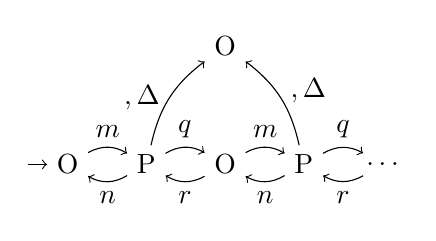
\begin{tikzpicture}[baseline=(O1.base)]
    \node (O1) at (0,0) {\kw{O}};
    \node (P1) at (1,0) {\kw{P}};
    \node (O2) at (2,0) {\kw{O}};
    \node (P2) at (3,0) {\kw{P}};
    \node (O3) at (4,0) {$\ldots$};
    \node (H) at (2,1.5) {\kw{O}};
    \path [->] (-0.5,0) edge (O1);
    \path [->] (O1) edge[bend left] node[auto] {$m$} (P1);
    \path [->] (P1) edge[bend left] node[auto] {$n$} (O1);
    \path [->] (P1) edge[bend left] node[auto] {$q$} (O2);
    \path [->] (P1) edge[bend left=20] node[auto,anchor=east] {$\lightning, \Delta$} (H);
    \path [->] (O2) edge[bend left] node[auto] {$r$} (P1);
    \path [->] (O2) edge[bend left] node[auto] {$m$} (P2);
    \path [->] (P2) edge[bend left] node[auto] {$n$} (O2);
    \path [->] (P2) edge[bend left] node[auto] {$q$} (O3);
    \path [->] (P2) edge[bend right=20] node[anchor=base west] {$\lightning, \Delta$} (H);
    \path [->] (O3) edge[bend left] node[auto] {$r$} (P2);
  \end{tikzpicture}
  \quad
  \begin{array}{c@{\,}lc@{\,}l}
    m &\in M_B^\kw{Q} & q &\in M_A^\kw{Q} \\[1ex]
    n &\in M_B^\kw{A} & r &\in M_A^\kw{A}
  \end{array}
\]
The first move is always a question $m$ played by $\kw{O}$ in $B$.
The player $\kw{P}$ can conclude the current instance of $B$
with an answer $n$, or
initiate an instance of $A$
with a question $q$.
Then $\kw{O}$ can initiate a new instance of $B$
with another $m$, or
conclude any current instance of $A$
with an answer $r$.
This process goes on indefinitely.

To formalize the plays and strategies of $A \rightarrow B$
in a way that accounts for refinement,
we decouple two aspects of this structure.
The following definition of plays
enforces the alternation between $\kw{O}$ and $\kw{P}$.

\begin{definition} % arrow game {{{
Given two elementary games $A$ and $B$,
the moves of the arrow game $A \rightarrow B$
are the questions and answers of $A$ and $B$,
categorized as follows:
\begin{align*}
  M_{A \rightarrow B}^\kw{O} &= M_A^\kw{A} + M_B^\kw{Q} &
  M_{A \rightarrow B}^\kw{Q} &= M_A^\kw{Q} + M_B^\kw{Q} \\
  M_{A \rightarrow B}^\kw{P} &= M_A^\kw{Q} + M_B^\kw{A} &
  M_{A \rightarrow B}^\kw{A} &= M_A^\kw{A} + M_B^\kw{A}
\end{align*}
The \emph{plays} are taken in
the prefix closure $P_{A \rightarrow B}$ of the set:
\[
    (M_{A \rightarrow B}^\kw{O}
     M_{A \rightarrow B}^\kw{P})^* \,
    (\varepsilon +
     M_{A \rightarrow B}^\kw{O} \Delta +
     M_{A \rightarrow B}^\kw{O} \lightning) \,.
\]
Note that
even-length plays represent positions where $\kw{O}$ is expected to play,
whereas odd-length plays represent positions where $\kw{P}$ is.
We write $P_{A \rightarrow B}^\kw{even}$ and $P_{A \rightarrow B}^\kw{odd}$
for the corresponding subsets of $P_{A \rightarrow B}$.
\end{definition}
%}}}

The ``stack discipline'' associating questions
with their eventual answer is captured by
the way we extend refinement conventions to
the plays of $A \rightarrow B$.

\begin{definition} % F_A->B %{{{
Given
$\mathbb{C}_A : \mathcal{R}(A_1, A_2)$ and
$\mathbb{C}_B : \mathcal{R}(B_1, B_2)$,
we can define the following relations
between the moves of $A_1 \rightarrow B_2$
and the moves of $A_2 \rightarrow B_2$:
\begin{align*}
  {\preceq}_{\mathbb{C}_A \rightarrow \mathbb{C}_B}^\kw{O} &=
    {\preceq}_{\mathbb{C}_A}^\kw{A} +
    {\preceq}_{\mathbb{C}_B}^\kw{Q} &
  {\preceq}_{\mathbb{C}_A \rightarrow \mathbb{C}_B}^\kw{Q} &=
    {\preceq}_{\mathbb{C}_A}^\kw{Q} +
    {\preceq}_{\mathbb{C}_B}^\kw{Q} \\
  {\preceq}_{\mathbb{C}_A \rightarrow \mathbb{C}_B}^\kw{P} &=
    {\preceq}_{\mathbb{C}_A}^\kw{Q} +
    {\preceq}_{\mathbb{C}_B}^\kw{A} &
  {\preceq}_{\mathbb{C}_A \rightarrow \mathbb{C}_B}^\kw{A} &=
    {\preceq}_{\mathbb{C}_A}^\kw{A} +
    {\preceq}_{\mathbb{C}_B}^\kw{A} \,,
\end{align*}
The Kripke frame
$\mathcal{F}_{\mathbb{C}_A \rightarrow \mathbb{C}_B} =
 \langle W_{\mathbb{C}_A \rightarrow \mathbb{C}_B}, \leadsto \rangle$
has worlds in
$W_{\mathbb{C}_A \rightarrow \mathbb{C}_B} =
 (W_{\mathbb{C}_A} + W_{\mathbb{C}_B})^*$,
and its accessibility relation $\leadsto$
relates moves of $A_1 \rightarrow B_1$
to moves of $A_2 \rightarrow B_2$,
as defined by the rules:
\[
    \AxiomC{$m_1 \ifr{w \Vdash {\preceq}_{\mathbb{C}_A \rightarrow \mathbb{C}_B}^\kw{Q}} m_2$}
    \UnaryInfC{$\vec{w} \stackrel{m_1, m_2}{\leadsto} w :: \vec{w}$}
    \DisplayProof
    \quad
    %\begin{array}{c}
    %  \vec{w} \stackrel{\#,\#}{\leadsto} \vec{w} \\[0.7ex]
    %  \vec{w} \stackrel{\tau, \tau}{\leadsto} \vec{w}
    %\end{array}
    %\quad
    \AxiomC{$m_1 \ifr{w \Vdash {\preceq}^\kw{A}_{\mathbb{C}_A \rightarrow \mathbb{C}_B}} m_2$}
    \UnaryInfC{$w :: \vec{w} \stackrel{m_1, m_2}{\leadsto} \vec{w} \,.$}
    \DisplayProof
\]
%Then two plays are related at $\vec{w}$
%when there is a path from $\varepsilon$ to $\vec{w}$
%in $\leadsto$ whose labels project onto the plays:
%\[
%    \AxiomC{$s : \varepsilon \leadsto^* \vec{w}$}
%    \UnaryInfC{$\pi_1^*(s)
%       \ifr{\vec{w} \Vdash {\preceq}_{A \rightarrow B}}
%       \pi_2^*(s)$}
%    \DisplayProof
%\]
%If
%$\langle A, \mathbb{C}_A \rangle$ and
%$\langle B, \mathbb{C}_B \rangle$
%are two games with refinement, then
%a \emph{valid play} of $A \rightarrow B$
%is a sequence $s \in P_{A \rightarrow B}$
%such that $(s, s) \in [\vec{w} \Vdash {\preceq}_{A \rightarrow B}]$
%for some $\vec{w}$.
\end{definition}

The frame $\mathcal{F}_{\mathbb{C}_A \rightarrow \mathbb{C}_B}$
is used in \S\ref{sec:sim}
to define our notion of simulation.
%}}}

%}}}

%}}}

\subsection{Strategies} %{{{

A strategy for $A \rightarrow B$
is essentially a tree
which gathers the possible interactions of
the system being modeled.
We give a traditional representation
as a prefix-closed set of plays,
but will work with strategies defined as transition systems.

\subsubsection{Traces} %{{{

In the existing literature,
strategies are usually formalized as prefix-closed sets of plays.
This establishes a connection with trace semantics of process calculi.
In our case,
a strategy given in this form is a set:
\[ \sigma \subseteq P_{A \rightarrow B} \,, \]
which satisfies
for all $st \in P_{A \rightarrow B}$
and $m \in M_{A \rightarrow B}^\kw{O}$:
\begin{itemize}
  \item $st \in \sigma \Rightarrow s \in \sigma$;
  \item $s\lightning \in \sigma \Rightarrow st \in \sigma$;
  \item $s \in \sigma \wedge sm \in P_{A \rightarrow B}
    \Rightarrow sm \in \sigma$.
\end{itemize}
The first condition ensures that $\sigma$ is prefix-closed.
It is complemented by the second condition,
which ensures that if a strategy goes wrong,
then it admits all other possible behaviors as well
from this point forward,
so that trace inclusion coincides with the notion of refinement
outlined in \S\ref{sec:bspec}.
The last condition ensures that
all possible behaviors of $\kw{O}$ are included
at all reachable positions.

%}}}

\subsubsection{Transition systems} %{{{

Instead of manipulating sets of traces directly,
we will define strategies using a specialized form of transition system.

\begin{definition} % strategy {{{
\label{def:strat}
An \emph{strategy} $\sigma$ for the arrow game $A \rightarrow B$
is a tuple
$\langle K, \delta, k_0 \rangle$
where:
\begin{itemize}
  \item $K$ is a set of \emph{continuation states};
  \item $\delta : K \rightarrow M_{A \rightarrow B}^\kw{O} \rightarrow
                  \mathcal{B}(M_{A \rightarrow B}^\kw{P} \times K)$
    specifies the behavior of each state
    for every possible opponent move;
  \item $k_0$
    is the strategy's \emph{initial continuation state}.
\end{itemize}
We write $\sigma : A \rightarrow B$ when $\sigma$ is a strategy
for $A \rightarrow B$.
\end{definition}
%}}}

Continuation states correspond to
the points in the execution where $\kw{O}$ is expected to move.
In reaction to an opponent move,
$\delta$ specifies which outcomes are possible:
the strategy may diverge, go wrong,
and specify successful outcomes
consisting of a proponent move,
together with a new continuation
which will be used to handle the next opponent move.

Accordingly,
the set of traces associated with a state is
defined recursively as:
\[
  \begin{array}{l@{\:}c@{\:\{}l@{\:\mid\:}l}
    \kw{traces}_\delta(k) & = & \varepsilon, m &
      m \in M_{A \rightarrow B}^\kw{O} \} \\
    & \cup & m \Delta &
      \delta(k, m) \ni \Delta \} \\
    & \cup & mt &
      \delta(k, m) \ni \lightning \wedge mt \in P_{A \rightarrow B} \} \\
    & \cup & m n t &
      \delta(k, m) \ni (n, k') \wedge t \in \kw{traces}_\delta(k') \}
  \end{array}
\]
Then the behavior of strategies can be made explicit
by specifying the corresponding sets of plays as:
\[
  \kw{traces}(\sigma) = \kw{traces}_\delta(k_0) \,.
\]

Formulated as transition systems,
the alternating structure of strategies
is ``baked into'' their definition.
This facilitates
mechanization in a proof assistant,
and facilitate a style of reasoning
which takes advantage of operational intuitions.

On the other hand,
in our approach strategies do not have a unique representation.
This is mitigated by the fact that
our primary concern will be refinement,
rather than equality of strategies:
we will mainly reason modulo simulations.

%}}}

%}}}

\subsection{Simulations} %{{{
\label{sec:sim}

Having formally defined a notion of strategy
for the game $A \rightarrow B$,
we turn to the corresponding relational notion of simulation
for the refinement convention $\mathbb{C}_A \rightarrow \mathbb{C}_B$.
To this end,
we first introduce the following modal constructions.

\begin{definition} % modal relators for simulation {{{
For frames labelled by pairs
($\Lambda = \Lambda_1 \times \Lambda_2$),
we define variants of $\Box, \Diamond$ which
allow world transitions to interact with the components
being related.
The relators:
\begin{align*}
  \Diamond \times {-} &: \mathcal{R}_W(A, B) \rightarrow
              \mathcal{R}_W(\Lambda_1 \times A, \, \Lambda_2 \times B) \\
  \Box \rightarrow - &: \mathcal{R}_W(A, B) \rightarrow
          \mathcal{R}_W(\Lambda_1 \rightarrow A, \, \Lambda_2 \rightarrow B)
\end{align*}
are defined as:
\begin{gather*}
  (l_1, a) \ifr{w \Vdash \Diamond \times R} (l_2, b) \Leftrightarrow
    a \ifr{w \Vdash \langle l_1, l_2 \rangle R} b \\
  f \ifr{w \Vdash \Box \rightarrow R} g \Leftrightarrow
    \forall \, l_1 l_2 \,.\, f(l_1) \ifr{w \Vdash [l_1, l_2] R} g(l_2)
\end{gather*}
\end{definition}
%}}}

With these constructions,
our notion of simulation relation
is naturally derived from
the type we used to define strategies (Def.~\ref{def:strat}).
They are used
with respect to the frame $\mathcal{F}_{A \rightarrow B}$
defined in \S\ref{sec:arrow}.
Hence, the simulation operates in the context of
a stack of elementary worlds
specifying how answers to pending questions
should be related.
In each one of the component games,
answers will be related at the same world as the corresponding questions:
$\kw{P}$ can rely on $\kw{O}$ making this true for the domain game;
it must guarantee that this is true for the codomain game.

\begin{definition} % simulation relation {{{
Given
$\mathbb{C}_A : \mathcal{R}(A_1, A_2)$,
$\mathbb{C}_B : \mathcal{R}(B_1, B_2)$
two refinement conventions, and
$\sigma_1 : A_1 \rightarrow B_1$,
$\sigma_2 : A_2 \rightarrow B_2$
two strategies,
a \emph{simulation relation} between $\sigma_1$ and $\sigma_2$
is a relation $R : \mathcal{R}_{W_{\!A \rightarrow B}}(K_1, K_2)$
such that:
\begin{gather*}
  \delta_1
  \ifr{\Vdash R \rightarrow \Box \rightarrow \mathcal{B}^+(\Diamond \times R)}
  \delta_2
  \\
  k_{0,1} \ifr{\varepsilon \Vdash R_K} k_{0,2}
\end{gather*}
We will write
$\sigma_1 \le_{\mathbb{C}_A \rightarrow \mathbb{C}_B}^R \sigma_2$
when $R$ is a simulation relation in this sense, and write
$\sigma_1 \le_{\mathbb{C}_A \rightarrow \mathbb{C}_B} \sigma_2$
when there exists any such simulation relation.
\end{definition}
%}}}

%}}}

\subsection{Constructions} %{{{

\subsubsection{Products} %{{{

The simplest way to aggregate a family of strategies $(\sigma_i)_{i \in I}$
is to annotate all of the moves by a component identifier $i$.
This corresponds to the categorical product.

\begin{definition} % Product game {{{
Given a family of elementary games $(A_i)_{i \in I}$,
we define their \emph{product} as the game:
\[ \prod_{i \in I} A_i =
   \Big\langle \sum_{i \in I} M_{A_i}^\kw{Q},
            \: \sum_{i \in I} M_{A_i}^\kw{A} \Big\rangle \,. \]
We will write $A_1 \times A_2 := \prod_{i \in \{1, 2\}} A_i$
and $A^I := \prod_{i \in I} A$.
\end{definition}
%}}}

The aggregated strategy uses the labels to direct each move
to the corresponding component,
and lets the components operate independently.

\begin{definition} % Product of strategies {{{
For a family of strategies
$(\sigma_i : A_i \rightarrow B_i)_{i \in I}$,
their product is the strategy
$\prod_i \sigma_i := \langle \prod_i K_i, \prod_i \delta_i, (k_i)_{i\in I} \rangle$,
where the relation
$\prod_i \delta_i$
is defined as:
\[
  (\vec{k}, (i, m)) \mapsto
    \delta_i(k_i, m) \bind (n, k_i') \mapsto ((i, n), \vec{k}[i := k_i']) \,.
\]
As before,
we write $\sigma_1 \times \sigma_2 := \prod_{i \in \{1, 2\}} \sigma_i$
and $\sigma^I := \prod_{i \in I} \sigma$.
\end{definition}
%}}}

%}}}

\subsubsection{Interaction} %{{{

While the product of two strategies
let them operate independently,
a construction like the composition $f \cdot g$ of
$f : A \rightarrow B$ and $g : B \rightarrow C$
is more subtle:
it involves the unbounded interaction of $f$ and $g$
over the common game $B$.

To model this interaction,
we introduce the following operator.
Given a strategy $\sigma : \Gamma \times A \rightarrow A \times \Delta$,
we will construct the strategy $Z(\sigma) : \Gamma \rightarrow \Delta$
by letting $\sigma$ interact with itself
over the game $A$ common to its domain and codomain.

\begin{definition}
Given $\sigma : \Gamma \times A \rightarrow A \times \Delta$,
we define the strategy $Z(\sigma) : \Gamma \rightarrow \Delta$
by iteration over the set of states:
\[
    S := K_\sigma \times (M_\Gamma + M_A + M_\Delta) \,.
\]
When a continuation of $Z(\sigma)$ is resumed by an opponent move,
we first store the move as a component of the state:
\begin{gather*}
  \kw{in} : K_\sigma \rightarrow
            M_{\Gamma \rightarrow \Delta}^\kw{O} \rightarrow
            \mathcal{B}(S) \\
  \kw{in}_k(m) := \{ (k, m) \}
\end{gather*}
Then, we will let $\sigma$ act on the state
by lifting its transition relation to $S$.
Given the obvious injections:
\begin{align*}
  \iota_\kw{O} &:
    M_{\Gamma \times A \rightarrow A \times \Delta}^\kw{O}
    \rightarrow
    M_\Gamma + M_A + M_\Delta \\
  \iota_\kw{P} &:
    M_{\Gamma \times A \rightarrow A \times \Delta}^\kw{P}
    \rightarrow
    M_\Gamma + M_A + M_\Delta \,,
\end{align*}
we define the relation
$\kw{step} : S \rightarrow \mathcal{B}(S)$
using the rule:
\[
  \kw{step}(k, \iota_\kw{O}(m)) =
    \delta_\sigma(k, m) \bind (m', k') \mapsto (k', \iota_\kw{P}(m')) \,,
\]
with the understanding that $\kw{step}(k, m) = \bot$
whenever the current move $m$ is
in $M_\Gamma^\kw{Q}$ or $M_\Delta^\kw{A}$.
When we reach such a move,
we instead return control to the environment:
\begin{gather*}
  \kw{out} : S \rightarrow
    \mathcal{B}(M_{\Gamma \rightarrow \Delta}^\kw{P} \times K) \\
  \kw{out}(k, m) =
    \{ (m, k) \mid m \in M_{A \rightarrow B}^\kw{P} \}
\end{gather*}
With these, the strategy $Z(\sigma)$ can be defined as:
\[
    Z(\sigma) := \langle
       K_\sigma, \:
       k \mapsto \kw{in}_k \cdot \kw{step}^* \cdot \kw{out}, \:
       k_{0\sigma}
     \rangle \,.
\]
\end{definition}

%}}}

\subsubsection{Identity and composition} %{{{

With products and the interaction combinator $Z$,
we can define the categorical composition of
$f : A \rightarrow B$ and $g : B \rightarrow C$ as:
\[
    f \cdot g := Z(f \times g) \,.
\]
The identity strategy $\kw{id}_A : A \rightarrow A$
simply passes codomain questions to the domain game,
and passes domain answers back to the codomain.
It is defined as:
$\kw{id}_A := \langle \{ * \}, \delta_\kw{id}, * \rangle$,
with $\delta_\kw{id}(*, m) = \{(m, *)\}$.

%}}}

\subsubsection{Duplication} %{{{

Although we have defined the product of strategies
$\prod_i \sigma_i : \prod_i A_i \rightarrow \prod_i B_i$,
we have not yet defined the tupling operation
$\langle \sigma_i \rangle_{i \in I}$
distinguishing the cartesian product
from weaker monoidal structures.
To this end,
we introduce the diagonal morphism
$\Delta_A^I : A \rightarrow A^I$.

The diagonal morphism simply passes through any
opponent question from a component $i \in I$ of its codomain
as a proponent question in its domain.
To make sure the answer can be routed back to $i$,
we remember which component of the codomain initiated
each pending question.
Hence,
the continuations of $\Delta$
consist of a stack $\iota \in I^*$
of component identifiers.

\begin{definition}[Diagonal morphism] % diagnoal morphism {{{
For an elementary game $A$ and a set $I$,
we define the strategy:
\[ \Delta_A^I := \langle I^*, \delta_\Delta, \varepsilon \rangle
  : A \rightarrow A^I \,. \]
Writing $m \in M_A^\kw{Q}$ and $n \in M_A^\kw{A}$,
the transition relation $\delta_\Delta$
is defined by the rules:
\begin{align*}
  \delta_\Delta(\iota, (i, m)) &\ni (m, i :: \iota) & m &\in M_A^\kw{Q} \\
  \delta_\Delta(i :: \iota, n) &\ni ((i, n), \iota) & n &\in M_A^\kw{A} \,.
\end{align*}
Then for a family of strategies $(\sigma_i : A \rightarrow B_i)_{i \in I}$,
we define
$\langle \sigma_i \rangle_{i \in I} : A \rightarrow \prod_i B_i$
as the strategy:
\[
    \langle \sigma_i \rangle_{i \in I} := 
      \Delta^I \cdot \prod_i \sigma_i \,.
\]
\end{definition}
%}}}

%}}}

\subsubsection{Choice} %{{{

Because our underlying notion of behavior supports
nondeterministic choice,
in addition to the diagonal morphism
$\Delta : A \rightarrow A^I$,
we can define a strategy
$\Sigma : A^I \rightarrow A$
which will pass each opponent question in the codomain
to a nondeterministically chosen component in the domain.

\begin{definition}
For an elementary game $A$ and a set $I$,
the strategy $\Sigma_A^I : A^I \rightarrow A$
is defined as $\langle \{*\}, \delta_\Sigma, * \rangle$
where $\delta_\Sigma$ is defined by the rules:
\begin{align*}
  &\delta_\Sigma(*, m) \ni \{((i, m), *)\} & m &\in M_A^\kw{Q} \\
  &\delta_\Sigma(*, (i, n)) \ni \{(n, *)\} & n &\in M_A^\kw{A} \,.
\end{align*}
For $f, g : A \rightarrow B$,
the strategy $f \oplus g$ is defined as:
\[ f \oplus g := \Delta \cdot (f \times g) \cdot \Sigma \,. \]
\end{definition}

This construction allows us to complement
the multiplicative structure $\langle \cdot, \kw{id} \rangle$
of our game model
with an additive component $\langle \oplus, \bot \rangle$.
The additive identity is defined as the empty strategy
$\bot_{A,B} := \langle \{*\}, * \mapsto 0, * \rangle : A \rightarrow B$.
The strategy $f \oplus g$
implements a form of continuous nondeterministic choice between $f$ and $g$:
for each incoming question in $M_B^\kw{Q}$,
the operator will nondeterministically route it to either $f$ or $g$.

%}}}

\subsubsection{Iterated composition}

The logical next step is to define the Kleene star
associated with $\cdot$ and $\oplus$.
Given a strategy $\sigma : A \rightarrow A$,
we define:
\begin{align*}
  \sigma^{\oplus} &:= Z(\Sigma \cdot \sigma \cdot \Delta) \\
  \sigma^{\oast} &:= \sigma^{\oplus} \oplus \kw{id}_A
\end{align*}

Once again,
the structure
$\langle \mathcal{G}[A,A], \cdot, \kw{id}, \oplus, \bot, {}^\oast \rangle$
does not define a Kleene algebra,
because $\bot$ may not act as an absorbing element
on the left of $\cdot$.
Nevertheless,
these operations will allow us to construct
more complex operators on strategies,
such as the horizontal composition of CompCert components
defined in \S\ref{sec:hcomp},
and to use equational reasoning to
establish properties of these operators.

%}}}

\subsection{Relational properties} %{{{

XXX: I want to show that all of the basic constructions
are compatible with simulations.
The junk below is outdated but contains
definitions of simulation relations that I should be able
to reuse.

{ \color{gray} %{{{

Furthermore,
for a refinement convention
$\mathbb{C} : \mathbb{R}_{W}(A_1, A_2)$,
the relation $R_\kw{id}$ defined by the single rule:
\[
    \AxiomC{$\vec{w} = w_1 w_1 \cdots w_n w_n$}
    \UnaryInfC{$* \ifr{\vec{w} \Vdash R_\kw{id}} *$}
    \DisplayProof
\]
is such that
$\kw{id}_{\!A_1} \le_{\mathbb{C} \rightarrow \mathbb{C}}^{R_\kw{id}} \kw{id}_{\!A_2}$.

\begin{definition}
For a family of refinement conventions
$(\mathbb{C}_i : \mathcal{R}(A_i, B_i))_{i \in I}$,
we define:
\[ \prod_{i \in I} \mathbb{C}_i =
   \langle W, {\preceq}^\kw{Q}, {\preceq}^\kw{A} \rangle :
   \mathcal{R}\Big(\prod_i A_i, \prod_i B_i \Big) \]
where
$W = \sum_i W_{\mathbb{C}_i}$ and
$\preceq^\kw{Q}, \preceq^\kw{A}$
are given by the rules:
\[
    \small
    \AxiomC{$m_1 \ifr{w \Vdash {\preceq}_{\mathbb{C}_i}^\kw{Q}} m_2$}
    \UnaryInfC{$(i, m_1) \ifr{(i, w) \Vdash {\preceq}^\kw{Q}} (i, m_2)$}
    \DisplayProof
    \quad
    \AxiomC{$m_1 \ifr{w \Vdash {\preceq}_{\mathbb{C}_i}^\kw{A}} m_2$}
    \UnaryInfC{$(i, m_1) \ifr{(i, w) \Vdash {\preceq}^\kw{A}} (i, m_2)$}
    \DisplayProof
\]
\end{definition}

\begin{lemma} % monotonicity {{{
For a family of simulation relations $\vec{R} = (R_i)_{i \in I}$ such that
$\sigma_{1,i} \le_{\mathbb{C}_A \rightarrow \mathbb{C}_B}^{R_i} \sigma_{2,i}$,
the relation $\mathcal{M}(\vec{R})$ defined by:
\begin{gather*}
  \AxiomC{$\forall i \,.\,
    k_{1,i} \ifr{\vec{w} \restriction i \Vdash R_{K,i}} k_{2,i}$}
  \UnaryInfC{$\vec{k_1} \ifr{\vec{w} \Vdash \mathcal{M}(\vec{R})_K} \vec{k_2}$}
  \DisplayProof
  \\[.5ex]
  \AxiomC{$s_1 \ifr{\vec{w} \restriction i \Vdash R_{S,i}} s_2$}
  \AxiomC{$\forall j \ne i \,.\,
    k_{1,j} \ifr{\vec{w} \restriction j \Vdash R_{S,j}} k_{2,j}$}
  \BinaryInfC{$(i, s_1, \vec{k}_1)
    \ifr{\vec{w} \Vdash \mathcal{M}(\vec{R})_S}
    (i, s_2, \vec{k}_2)$}
  \DisplayProof
\end{gather*}
is a simulation relation between the strategies:
\[
  \mathcal{M}(\vec{\sigma_1})
  \le_{\mathbb{C}_A^I \rightarrow \mathbb{C}_B^I}^{\mathcal{M}(\vec{R})}
  \mathcal{M}(\vec{\sigma_2}) \, .
\]
The stack of worlds $\vec{w} \restriction i$
is the sequence $w_1, w_2, \ldots, w_n$
such that $(i, w_1), (i, w_2), \ldots, (i, w_n)$
is the subsequence of $\vec{w}$ containing worlds
paired with $i$ indices.
\end{lemma}
%}}}

\subsubsection{Flat composition} %{{{

Once we have such an aggregate,
we can ``flatten'' the communication between
the system and the environment
back to the unannotated game $A \rightarrow B$.

\begin{definition} % flattening {{{
The \emph{flattening} of $\sigma : A^I \rightarrow B^I$
is the strategy $\sigma^\rhd : A \rightarrow B$
defined over the sets of states
$K := K_\sigma \times I^*$ and
$S := S_\sigma \times I^*$ by the following rules:
\[
  \begin{array}{c@{\quad}c}
    \AxiomC{$k \xrightarrow{(i, m)}_\sigma s$}
    \AxiomC{$\forall \, j \ne i \,.\, k \: \#_{\!\sigma} \: (j, m)$}
    \BinaryInfC{$(k, \iota) \xrightarrow{m} (s, \iota)$}
    \DisplayProof
    &
    \AxiomC{$s \xrightarrow{(i, n)}_\sigma k$}
    \UnaryInfC{$(s, \iota) \xrightarrow{n} (k, \iota)$}
    \DisplayProof
    \\[1.5em]
    \AxiomC{$s \xrightarrow{(i, q)}_\sigma k$}
    \UnaryInfC{$(s, \iota) \xrightarrow{q} (k, i :: \iota)$}
    \DisplayProof
    &
    \AxiomC{$k \xrightarrow{(i, r)}_\sigma s$}
    \UnaryInfC{$(k, i :: \iota) \xrightarrow{r} (s, \iota)$}
    \DisplayProof
    \\[1.5em]
    \AxiomC{$s \xrightarrow{\tau}_\sigma s'$}
    \UnaryInfC{$(s, \iota) \xrightarrow{\tau} (s', \iota)$}
    \DisplayProof
    &
    \AxiomC{$\forall \,i\,.\, k \: \#_{\!\sigma} \: (i, m)$}
    \UnaryInfC{$(k, \iota) \:\#\: m$}
    \DisplayProof
  \end{array}
\]
\end{definition}
%}}}

We direct an incoming question in $B$
to a component $i$ when all other components reject it.
If the component then asks a question in the game $A$,
we save its identifier on the stack $\iota$,
so that the corresponding answer can be directed back to $i$.

\begin{lemma}
Given a simulation relation
$\sigma_1 \le_{\mathbb{C}_A^I \rightarrow \mathbb{C}_B^I}^R \sigma_2$,
the relation $R^\rhd$ is defined for continuation states by:
\[
  \AxiomC{$k_1 \ifr{\vec{w} \Vdash R_K} k_2$}
  \AxiomC{$\iota = \pi_1^*(\vec{w}) \mbox{ XXX}$}
  \BinaryInfC{
    $(k_1, \iota) \ifr{\pi_2^*(\vec{w}) \Vdash R^\rhd_K} (k_2, \iota)$}
  \DisplayProof
\]
and similarly for running states.
$R^\rhd$ is a simulation relation:
\[
    \sigma_1^\rhd
    \le_{\mathbb{C}_A \rightarrow \mathbb{C}_B}^{R^\rhd}
    \sigma_2^\rhd \,.
\]
\end{lemma}

Putting together multi-component strategies and flattening,
the \emph{flat composition} operator
$\mathcal{F} : [A \rightarrow B] \rightarrow [A \rightarrow B]$
is:
\[
    \mathcal{F}(\vec{\sigma}) := \mathcal{M}(\vec{\sigma})^\rhd
\]
This allows us to bundle multiple components of the same type,
however note that so far they do not interact with each other
(only to decide who's going to handle what question).

%}}}

\subsubsection{Resolution operator} %{{{

To allow interaction within a composite system,
we define the following resolution operator,
which feeds back a strategy's own questions to itself
whenever possible.

\begin{definition} % resolution {{{
The \emph{resolution} of $\sigma : A \rightarrow A$,
written $\mathcal{R}(\sigma)$,
is defined over the sets of states
$K := K_\sigma \times \{\kw{O}, \kw{P}\}^*$ and
$S := S_\sigma \times \{\kw{O}, \kw{P}\}^*$
by the following rules:
\[
  \begin{array}{cc}
    {\small m \in M_A^\kw{Q}, \:\: n \in M_A^\kw{A}}
    &
    {\small q \in M_A^\kw{Q}, \:\: r \in M_A^\kw{A}}
    \\[1em]
    \AxiomC{$k \xrightarrow{m}_\sigma s$}
    \UnaryInfC{$(k, \iota) \xrightarrow{m} (s, \kw{O} :: \iota)$}
    \DisplayProof
    &
    \AxiomC{$s \xrightarrow{n}_\sigma k$}
    \UnaryInfC{$(s, \kw{O} :: \iota) \xrightarrow{n} (k, \iota)$}
    \DisplayProof
    \\[1.5em]
    \AxiomC{$s \xrightarrow{q}_\sigma k$}
    \AxiomC{$k \:\#_{\!\sigma}\: q$}
    \BinaryInfC{$(s, \iota) \xrightarrow{q} (k, \iota)$}
    \DisplayProof
    &
    \AxiomC{$k \xrightarrow{r}_\sigma s$}
    \UnaryInfC{$(k, \iota) \xrightarrow{r} (s, \iota)$}
    \DisplayProof
    \\[1.5em]
    \AxiomC{$s \xrightarrow{q}_\sigma k$}
    \AxiomC{$k \xrightarrow{q}_\sigma s'$}
    \BinaryInfC{$(s, \iota) \xrightarrow{\tau} (s', \kw{P} :: \iota)$}
    \DisplayProof
    &
    \AxiomC{$s \xrightarrow{r}_\sigma k$}
    \AxiomC{$k \xrightarrow{r}_\sigma s'$}
    \BinaryInfC{$(s, \kw{P} :: \iota) \xrightarrow{\tau} (s', \iota)$}
    \DisplayProof
    \\[1.5em]
    \AxiomC{$s \xrightarrow{\tau}_\sigma s'$}
    \UnaryInfC{$(s, \iota) \xrightarrow{\tau} (s', \iota)$}
    \DisplayProof
    &
    \AxiomC{$k \:\#_{\!\sigma}\: m$}
    \UnaryInfC{$(k, \iota) \:\#\: m$}
    \DisplayProof
  \end{array}
\]
The initial continuation is $(k_{\sigma}, \varepsilon)$.
\end{definition}
%}}}

\begin{lemma}
If
$\sigma_1 \le_{\mathbb{C}_A \rightarrow \mathbb{C}_A}^R \sigma_2$,
then
$\mathcal{R}(\sigma_1)
 \le_{\mathbb{C}_A \rightarrow \mathbb{C}_A}^{\mathcal{R}(R)}
 \mathcal{R}(\sigma_2)$,
where $\mathcal{R}(R)$ is defined as follows.
For a world $\vec{w} \in W_{A \rightarrow B}$
and a stack $\iota \in \{\kw{O}, \kw{P}\}^*$,
the set $\mathcal{R}_\iota(\vec{w}) \subseteq W_{A \rightarrow B}$
is defined by the following rules together with the base case
$\varepsilon \in \mathcal{R}_\varepsilon(\varepsilon)$:
\[
    \AxiomC{$\vec{w}' \in \mathcal{R}_\iota(\vec{w})$}
    \UnaryInfC{$x :: \vec{w}' \in \mathcal{R}_{\kw{O} :: \iota}(x :: \vec{w})$}
    \DisplayProof
    \quad
    \AxiomC{$\vec{w}' \in \mathcal{R}_\iota(\vec{w})$}
    \UnaryInfC{$x :: x :: \vec{w}' \in \mathcal{R}_{\kw{P} :: \iota}(\vec{w})$}
    \DisplayProof
\]
XXX this is only the rules for codomain worlds,
we need a case for domain worlds to be passed along.

Then the relation $\mathcal{R}(R)$ is given for continuation states by:
\[
  \AxiomC{$k_1 \ifr{\vec{w} \Vdash R_K} k_2$}
  \AxiomC{$\vec{w}' \in \mathcal{R}_\iota(\vec{w})$}
  \BinaryInfC{$(k_1, \iota) \ifr{\vec{w}' \Vdash \mathcal{R}(R)_K} (k_2, \iota)$}
  \DisplayProof
\]
and similarly for running states.

XXX the proof needs $\mathcal{R}(\vec{w})$ to take into account
whether the component is currently running (states) or not (continuations).
\end{lemma}

%}}}

\subsubsection{Observation operator} %{{{

The simulations defined in \S\ref{sec:sim}
only relate strategies whose internal actions match one-to-one.
However, the operator defined in this section
will allow us to normalize strategies by removing
all finite sequences of $\tau$s.

\begin{definition}
Given $\sigma : A \rightarrow B$,
the \emph{observation strategy}
$\sigma \backslash \tau^* =
 \langle K_\sigma, S_\sigma \uplus \{\ast\},
         \xrightarrow{\kw{O}},
         \xrightarrow{\tau},
         \xrightarrow{\kw{P}}_\sigma,
         \#_\sigma, k_{0,\sigma} \rangle$
uses the resumption and internal transition relations
defined by the rules:
\[
  \AxiomC{$s \xrightarrow{\tau}_\sigma s'$}
  \AxiomC{$s' \xrightarrow{\tau^\omega}$}
  \doubleLine \BinaryInfC{$s \xrightarrow{\tau^\omega}$}
  \DisplayProof
  \qquad
  \AxiomC{$k \xrightarrow{m}_\sigma s$}
  \AxiomC{$s \xrightarrow{\tau^\omega}$}
  \BinaryInfC{$k \xrightarrow{m} \ast$}
  \DisplayProof
\]\[
  \AxiomC{$k \xrightarrow{m}_\sigma s$}
  \AxiomC{$s \xrightarrow{\tau^*}_\sigma s' \xrightarrow{n}_\sigma k'$}
  \BinaryInfC{$k \xrightarrow{m} s'$}
  \DisplayProof
  \qquad
  \ast \xrightarrow{\tau} \ast \,.
\]
\end{definition}

\begin{lemma}
If $\sigma_1 \le_{\mathbb{C}_A \rightarrow \mathbb{C}_B}^R \sigma_2$,
then for $R \backslash \tau^* = R \cup \{(\ast, \ast)\}$
the following holds:
\[
  \sigma_1 \backslash \tau^*
  \le_{\mathbb{C}_A \rightarrow \mathbb{C}_B}^{R \backslash \tau^*}
  \sigma_2 \backslash \tau^* \,.
\]
\end{lemma}

%}}}

Note that for both states and continuations,
nondeterminism is interpreted as \emph{output} nondeterminism,
as prescribed by the use of the relator $\mathcal{P}^+$.
This means that alternating transition system
implicitely accept all possible inputs from the environment,
although some of them may cause the system to immediately go wrong.
Likewise,
the special resumption $\kw{refuse}$
is taken as a positive, output behavior from the system,
rather than a restriction on the environment ---
this will be important to establish the monotonicity
of the composition operator defined in Sec.~\ref{?}.
This approach corresponds to the saturation requirement on strategies
often found in traditional game semantics,
or notions of receptiveness used in CompCert
and in concurrency theory.

Furthermore, we need to distinguish between mere nondeterminism
and \emph{branching}.
This is explored in the following section.

\subsection{Branching and determinism}

Whereas nondeterminism allows a strategy to posess
multiple observable behaviors,
branching occurs when multiple state transitions
are associated with the same immediate observable behavior.
This can create spurious distinctions,
whereby systems that yield the same sets of traces
cannot be identified by simulation,
and as such we consider it undesirable.
The following definition
formalizes the conditions a transition system must satisfy
to be considered free from branching.

\begin{definition}[Nonbranching transition system]
For given sets of moves and states,
a continuation $k : M \rightarrow \mathcal{P}(\kw{resumption}(S))$
is \emph{nonbranching} if the following property holds:
\[ \forall m \,.\, | k(m) | \le 1 \]
A transition system $\alpha : \kw{ats}(M, S)$ is nonbranching
if the following property holds:
\[ \forall s, m, k_1, k_2 \,.\,
     \alpha(s) \supseteq \{ m \cdot k_1, m \cdot k_2 \} \Rightarrow
     k_1 = k_2 \,, \]
and if for all $s, m, k$ such that $\alpha(s) \ni \underline{m} \cdot k$,
the continuation $k$ is nonbranching.
\end{definition}

Determinism is a stronger property,
and ensures that the system has at most one possible behavior
at any point.
We expect the semantics of concrete systems ---
as opposed to specifications ---
to be deterministic in the following sense.

\begin{definition}[Deterministic transition system]
For given sets of moves and states,
a transition system $\alpha : \kw{ats}(M, S)$
is deterministic if for all $s$, $|\alpha(s)| \le 1$,
and if for all $s, m, k$ such that $\alpha(s) \ni \underline{m} \cdot k$,
the continuation $k$ is nonbranching.
\end{definition}

Note that both nonbranching and determinism
only relate to the behavior of the system.
In both cases,
the environment remains free to play any move.
Abramsky notes in \cite{cspgs}
that [it's one of the good things about game semantics].

\subsection{Internal actions and divergence}

The emergence of silent divergence
is one of the major difficulties
associated with modeling interacting systems.
Indeed,
two systems which, taken in isolation,
only exhibit reactive behavior,
can nonetheless become silently divergent when composed together,
if it is possible to interact with each other continuously
without intervening communication with the outside.

An operational description of this phenomenon
models this internal interaction explicitly
in the form of silent actions $\tau$.
When comparing the behavior of two systems,
finite sequences of $\tau$'s will be considered equivalent.
However,
silent divergence in the form of an infinite sequence of $\tau$'s
can only correspond to another infinite sequence.
This is usually addressed by the introduction of
sophisticated notions of simulation,
such as the \emph{measure simulations} used for instance in CompCert.

On the other hand,
in most work on denotational semantics,
including traditional game semantics such as \cite{pcfgs},
[complicated fixpoints] 

Our model includes a notion of internal action $\tau$,
which makes it possible to handle silent divergence explicitely
rather than through sophisticated domain-theoretic constructions.
However,
note that the notion of simulation we have defined
does not allow any variation
in the number of internal transitions
between the two transition systems being related.
Nevertheless,
composition operators remain monotonic
under this definition of simulation,
because [...]
Normalize using the following operator.

\begin{definition}[Observation operator]
For a transition system $\alpha : \kw{ats}(M, S)$,
we define the \emph{observations} transition system
$\mathcal{O}(\alpha)$ as follows.
A behavior $r : \kw{behavior}(M, S)$ is said to be
\emph{observable} if $r \ne \tau \cdot s$ for all $s \in S$.
A state $s' \in S$ is said to be \emph{reachable} from $s \in S$
if there is a sequence $s_0, s_1, \ldots s_n$ such that
$s_0 = s$, $s_n = s'$,
and for all $0 \le i < n$
there is a transition $\alpha(s_i) \ni \tau \cdot s_{i+1}$.
A state $s$ is said to be \emph{silently divergent}
if there is an infinite sequence $s_0, s_1, \ldots$
such that $s_0 = s$ and for all $i$,
there is a transition $\alpha(s_i) \ni \tau \cdot s_{i+1}$.
Then the observations transition system is defined as:
\begin{align*}
    \mathcal{O}(\alpha)(s) = &\{ r \:|\: r \mbox{ is observable } \wedge
         \exists s' \,.\, s \rightarrow^* s' \wedge
		\alpha(s') \ni r \} \\
      \cup &\{ \Delta \:|\: s \mbox{ is silently divergent} \}
\end{align*}
\end{definition}

Properties:
preserve nonbranching (if that's defined in the right way), determinism.
Monotonic.

}
%}}}
